\chapter{Bayesian quantile-based correction and synthesis of hydrologic products}
\label{ch:research-b}

\section{Forecasting problem and contribution}

River-flow forecasts support flood preparedness, drought monitoring, reservoir
operations, and water-supply planning. These decisions require predictive
distributions that describe routine conditions and extremes. Hydrological
uncertainty arises from imperfect observations, model structure, parameters,
and initial states. Meteorological uncertainty enters through precipitation
and other atmospheric forcing as weather inputs propagate through a catchment
\citep{env-thiboult2016accounting,env-tarek2021daily}. Operational forecasts
use conceptual and physically based hydrological models whose calibration and
implementation shape this propagation \citep{env-demargne2013science}.
Statistical correction must therefore relate model output to flow observed at
a gauge while preserving the uncertainty relevant to prediction.

Forecast combination and statistical post-processing provide established
approaches to this problem \citep{env-siegert2019forecast,env-vannitsem,
env-wang2022forecastcombinations50yearreview}. Bayesian model averaging has
been used to combine hydrological predictive distributions
\citep{env-duan2006bma}; ensemble model output statistics (EMOS) relates
distribution parameters to ensemble forecasts \citep{env-gneiting2005emos},
including location and spread corrections in hydrology
\citep{env-hemri2015multivariate}. Quantile methods have been used to merge
precipitation products \citep{env-yumnam2022quantile}, and dynamic Bayesian
predictive synthesis combines information over time
\citep{env-mcalinn2019dynamic}. The setting considered here differs because
the available products have different spatial support, update frequencies,
and forecast horizons, and because retrospective products and issued
ensembles play distinct statistical roles.

Within dynamic quantile linear models (DQLMs;
\citealp{env-gourieroux2008dqlm,env-goncalves,exd-me}), this chapter makes
three contributions. First, a shared latent quantile process relates gauge
measurements to retrospective products and issued ensembles through
source-specific dynamic discrepancies. This separates a common river-flow
signal from persistent product-specific departures while allowing source
availability to vary by lead. Second, predictive synthesis combines the full
predictive distributions from separately fitted quantile models, including
their tails, into a nondecreasing marginal quantile function. Third, a
Laplace--Delta variational approximation provides joint nonconjugate updates
of the scale and skewness parameters in the extended DQLM. The first two
contributions address the hydrologic combination problem; the third supplies
the computation needed for repeated fits to a multi-decade daily record.
These contributions extend, rather than replace, the DQLM and extended
asymmetric Laplace foundations cited above.

The application concerns daily San Lorenzo River flow at Big Trees,
California. It combines U.S. Geological Survey (USGS) observations with
European Centre for Medium-Range Weather Forecasts (ECMWF) Global Flood
Awareness System (GloFAS) products and National Oceanic and Atmospheric
Administration (NOAA) National Weather Service (NWS) products. Five forecast
origins provide 28-day and common eight-day comparisons using the continuous
ranked probability score (CRPS), targeted quantile losses, and predictive
calibration.

\section{Forecasting setting and data}
\label{env:sec:data}

\subsection{Study setting and observations}

The target is daily mean San Lorenzo River discharge at the USGS Big Trees
gauge, station 11160500, Santa Cruz, California
\citep{env-usgs_daily_11160500}. The record contains 12,995 daily observations
from May 29, 1987 through December 25, 2022. Discharge is converted from cubic
feet per second to m$^3$/s and modeled as $\log(1+x)$, where $x$ is discharge
in m$^3$/s. The record spans prolonged dry conditions and winter high-flow
episodes (Figure~\ref{env:fig:sanlorenzo}).

\begin{figure}[!htbp]
\centering
\includegraphics[width=0.95\textwidth]{figures/ch03-environ/site_context_usgs.png}
\caption[San Lorenzo River discharge at Big Trees]{USGS daily discharge, May
29, 1987 through December 25, 2022, on the $\log(1+x)$ scale with $x$ in
m$^3$/s. Dashed lines are approximate current-rating discharge equivalents of
current NWS minor and major stage categories at BTEC1/USGS 11160500, computed
from USGS rating 40.0 \citep{env-cnrfc_btec1,env-usgs_11160500_rating40}.
They provide magnitude references rather than historical flood-stage
classifications of daily means.}
\label{env:fig:sanlorenzo}
\end{figure}

A forecast origin, or cutoff, is denoted by $T$; the first verification date
is $T+1$. Paired gauge and retrospective records estimate each source's
discrepancy before $T$. External ensembles then inform future flow through the
discrepancy-adjusted source channels. Precipitation, soil moisture, and a
climate summary enter a separate transfer component of the latent quantile
process.

\subsection{External products and covariates}

The base transfer inputs are local precipitation from the Parameter-elevation
Regressions on Independent Slopes Model (PRISM) Climate Group
\citep{env-prism}, soil moisture from ECMWF ERA5-Land
\citep{env-ecmwf,env-munozsabater2021era5land}, and broader climate
information. Historical precipitation and soil moisture are extracted at the
gauge location; forecast-window paths include Global Ensemble Forecast System
precipitation and shallow soil-water forecasts. ERA5-Land supplies a
reanalysis-based land-state covariate, while USGS discharge supplies the
verification target.

Monthly NOAA Physical Sciences Laboratory climate-index series
\citep{env-noaa_climate_indices} are interpolated to daily resolution and
standardized. Their first generalized dynamic principal component
\citep{env-JSSv092c02} explains 44.07\% of total index variability and provides
the climate covariate. The product versions, spatial extraction rules, and
complete index list are recorded with the analysis materials
\citep{env-deleon2026sanlorenzo_reproducibility}.

GloFAS \citep{env-harrigan2020glofas} and NWS, including NOAA National Water
Model output \citep{env-cosgrove2024noaa}, each contribute a retrospective
discharge series and an issued ensemble. GloFAS has 51 members over 28 days.
The NWS ensemble has seven members: six extend to 8.5 days and one control to
ten days; the daily analysis retains eight valid leads. Source availability
determines which channels enter at each lead.

\section{Bayesian correction and predictive synthesis}
\label{env:sec:methodology}

For each target probability $p_0$, dynamic correction combines source channels
within a quantile fit; synthesis combines predictive distributions across
fits. We distinguish the conditional model quantile given states and
likelihood parameters, a posterior predictive quantile integrating their
uncertainty, and the synthesized predictive quantile. Bold symbols denote
vectors or matrices; $\mathbf I_r$, $\mathbf 0_r$, and $\mathbf 1_r$ denote
the $r$-dimensional identity, zero vector, and one vector.

\subsection{Quantile likelihood}
\label{env:subsec:exal}

The asymmetric Laplace (AL) distribution provides a working likelihood for
Bayesian quantile inference \citep{env-yu2001bayesian,
env-sriram2013theoretical}. We use the extended asymmetric Laplace (exAL)
distribution, $\operatorname{exAL}_{p_0}(\mu,\sigma,\gamma)$, developed by
\citet{exd-yan2025family}. Its location $\mu$ is the $p_0$-quantile,
$\sigma>0$ controls scale, and $\gamma$ provides additional skewness
flexibility. To preserve the specified quantile, $\gamma$ lies in an interval
$(L_\gamma(p_0),U_\gamma(p_0))$ whose endpoints depend on $p_0$.
Appendix~\ref{env:app:augmentation} records the endpoints and the conditional
Gaussian augmentation used in computation.

\subsection{State-space model}
\label{env:subsec:fullmodel}

The transformed-discharge process spans the observation period and forecast
horizon. The shared trend and seasonal state is
$\boldsymbol\theta_t\in\mathbb R^p$, with loading
$\mathbf F_t\in\mathbb R^p$. Each source
$j\in\mathcal J=\{1,\ldots,J\}$ has a discrepancy state
$\boldsymbol\delta_t^j\in\mathbb R^p$. A scalar transfer state $\zeta_t$
incorporates covariates $\mathbf x_t\in\mathbb R^m$ with time-varying
coefficients $\boldsymbol\psi_t\in\mathbb R^m$. Source $j$ has members
$i\in\mathcal I_j$ and leads $k\in\mathcal K_j$; let
$K_{\max}=\max_j K_{(j)}$.

Write $y_t^o$ for gauge observations, $z_t^j$ for retrospective source
discharge, and $y_T^{j,i}(k)$ for member $i$'s forecast issued at $T$ for lead
$k$, all on the $\log(1+x)$ scale. Conditional on states and channel
parameters, the observation channels are independent:
\begingroup\small
\begin{align}
y_t^o
&\sim \operatorname{exAL}_{p_0}
  (\mathbf F_t'\boldsymbol\theta_t+\zeta_t,\sigma^0,\gamma^0),
&&1\le t\le T, \label{env:eq:unified_usgs}\\
z_t^j
&\sim \operatorname{exAL}_{p_0}
  (\mathbf F_t'(\boldsymbol\theta_t+\boldsymbol\delta_t^j)+\zeta_t,
   \sigma^j,\gamma^j),
&&j\in\mathcal J,\ 1\le t\le T, \label{env:eq:unified_retro}\\
y_T^{j,i}(k)
&\sim \operatorname{exAL}_{p_0}
  (\mathbf F_{T+k}'(\boldsymbol\theta_{T+k}+\boldsymbol\delta_{T+k}^j)
   +\zeta_{T+k},\sigma^j,\gamma^j), \notag\\[-0.4ex]
&\hspace{7em}j\in\mathcal J,\quad i\in\mathcal I_j,
\quad k\in\mathcal K_j, \notag\\
\boldsymbol\theta_t\mid\boldsymbol\theta_{t-1}
&\sim \mathcal N(\mathbf G_t\boldsymbol\theta_{t-1},\mathbf W_t^\theta),
&&1\le t\le T+K_{\max}, \label{env:eq:unified_theta}\\
\boldsymbol\delta_t^j\mid\boldsymbol\delta_{t-1}^j
&\sim \mathcal N(\mathbf G_t\boldsymbol\delta_{t-1}^j,
                  \mathbf W_t^{\delta^j}),
&&j\in\mathcal J,\ 1\le t\le T+K_{\max}, \label{env:eq:unified_delta}\\
\zeta_t\mid\zeta_{t-1},\boldsymbol\psi_{t-1}
&\sim \mathcal N(\lambda\zeta_{t-1}+\mathbf x_t'\boldsymbol\psi_{t-1},
                  w_t^\zeta),
&&1\le t\le T+K_{\max}, \label{env:eq:unified_transfer}\\
\boldsymbol\psi_t\mid\boldsymbol\psi_{t-1}
&\sim \mathcal N(\boldsymbol\psi_{t-1},\mathbf W_t^\psi),
&&1\le t\le T+K_{\max}. \notag
\end{align}
\endgroup

The conditional gauge quantile is
$\mu^o_{p_0,t}=\mathbf F_t'\boldsymbol\theta_t+\zeta_t$; source quantiles
add $\mathbf F_t'\boldsymbol\delta_t^j$. The transition $\mathbf G_t$ and
covariances $\mathbf W_t^\theta,\mathbf W_t^{\delta^j}$ are $p\times p$,
$\mathbf W_t^\psi$ is $m\times m$, and $w_t^\zeta>0$ is scalar. The
persistence parameter $\lambda$ and $\mathbf x_t'\boldsymbol\psi_{t-1}$
govern the transfer update; $\mathbf x_{T+k}$ is the supplied lead-$k$
covariate vector.

Historical channels comprise the gauge and retrospective products; future
channels comprise available forecast members. Shared states induce dependence
after integration, although the working likelihood assumes conditionally
independent member residuals. Member counts, source scales, and augmentation
precisions jointly determine information contributions; there is no fixed
source-weight ratio. Retrospective and forecast products share
source-specific scale and skewness without a lead index. Residual member
correlation and lead-dependent observation scales are not explicitly modeled.

For prior specification and computation, stack the components as
\[
\boldsymbol\eta_t'=[\boldsymbol\theta_t',
(\boldsymbol\delta_t^1)',\ldots,(\boldsymbol\delta_t^J)',
\zeta_t,\boldsymbol\psi_t'],\qquad q=(J+1)p+m+1.
\]
Appendix~\ref{env:app:stackedstates} gives the corresponding selectors and
block matrices.

\subsection{Prior specification and discounting}
\label{env:subsec:prioranddisc}

Following \citet{exd-me}, assign channel-specific truncated Student-$t$
skewness priors and inverse-gamma scale priors,
\[
\gamma^s\sim t_{(L_\gamma(p_0),U_\gamma(p_0))}(0,\phi^s,\nu^s),
\qquad
\sigma^s\sim IG(a_{\sigma^s},b_{\sigma^s}),
\qquad s\in\mathcal J_0,
\]
where $\mathcal J_0=\{0\}\cup\mathcal J$ and channel 0 denotes the gauge.
Initialize $\boldsymbol\eta_0\sim\mathcal N(\mathbf m_0,\mathbf C_0)$.
Component discount factors \citep{env-prado2021time} control evolution
variances: values closer to one imply less adaptation. During forecasting, an
inverse-Wishart prior stabilizes evolution covariance around
$c\mathbf W_T$. Its posterior mean gives the origin covariance weight
$\epsilon/(1+\epsilon)$ and the expected state-innovation covariance weight
$1/(1+\epsilon)$. Appendix~\ref{env:app:forecastcovariance} provides the
active-state specification.

\subsection{Posterior computation}
\label{env:subsec:postinf}
\label{environ:sec:body-computation}

The AL and exAL fits use mean-field variational Bayes (VB); Gaussian variants
use Gaussian filtering and smoothing. Conditional Gaussian augmentation
permits variational filtering and smoothing for the state trajectory.
Coordinate ascent alternates state updates, observation-specific
augmentation updates, and joint scale--skewness updates. For the last block,
VB Laplace--Delta matches a mode and curvature on an unconstrained
parameterization; a second-order Delta approximation supplies nonlinear
expectations \citep{exd-wang2013nonconjugatevb}.
Appendix~\ref{app:hydrology-technical}, especially
Section~\ref{env:app:vblad}, states the factorization and update boundary.

This computation extends the importance-sampling treatment in \citet{exd-me},
which fixes the scale using an AL fit, by approximating scale and skewness
jointly. For the full record, a 34-dimensional state, and seven quantile
models, a full-data Markov chain Monte Carlo (MCMC) analysis is expected to
require several weeks because it repeatedly samples latent trajectories,
observation-specific augmentation variables, and nonconjugate parameters.
This is an estimate, not a measured MCMC comparison. Parallel VB computation
with \texttt{exdqlm} gives a representative combined fitting and forecasting
time of approximately two hours on the stated server configuration. A
matched full-model MCMC comparison has not been performed, so the predictive
assessments do not quantify variational posterior approximation error.

\subsection{Predictive synthesis across quantiles}
\label{env:subsec:quantilesynthesis}

The source-specific model is fitted separately at probabilities
$0<\tau_1<\cdots<\tau_L<1$, setting $p_0=\tau_\ell$ in fit $\ell$. These
fits need not produce ordered predictive quantiles. Let
$Y_{\ell,t}^{(r)}$, $r=1,\ldots,R$, denote predictive draws from fit $\ell$,
and let $q_{\ell,t}$ be their empirical $\tau_\ell$-quantile. Isotonic
regression first orders these quantiles \citep{exd-barlow1972}:
\[
\mathbf m_t^*=\underset{m_1\le\cdots\le m_L}{\arg\min}
\sum_{\ell=1}^L(q_{\ell,t}-m_\ell)^2.
\]
Each fit's draws are shifted by $m_{\ell,t}^*-q_{\ell,t}$. If
$Q^{\mathrm{adj}}_{\ell,t}$ is the empirical quantile function of the
shifted draws, then for $\tau_\ell<u<\tau_{\ell+1}$,
\[
Q_t^{\mathrm{init}}(u)=(1-w)Q^{\mathrm{adj}}_{\ell,t}(u)
+wQ^{\mathrm{adj}}_{\ell+1,t}(u),\qquad
w=\frac{u-\tau_\ell}{\tau_{\ell+1}-\tau_\ell}.
\]
Below $\tau_1$ and above $\tau_L$, the construction uses the adjusted
quantile functions from the outer fits. It therefore uses their predictive
tails as well as their fitted-probability quantiles.

The initial curve is evaluated on a dense probability grid and monotonically
rearranged \citep{exd-chernozhukov2010} to obtain a nondecreasing quantile
function $\widetilde Q_t$. Inverse-CDF sampling gives
\[
\widetilde Y_t^{(r)}=\widetilde Q_t(U_t^{(r)}),\qquad
U_t^{(r)}\sim\operatorname{Uniform}(0,1).
\]
We generate 2,000 draws per time. The outer fitted distributions supply tails
beyond probabilities 0.05 and 0.95, including central 95\% interval limits;
no separate 0.025 or 0.975 models are fitted. Synthesis specifies marginal
predictive distributions in time, not a joint temporal dependence model for
sample traces. Appendix~\ref{env:app:numericalprediction} records the grid,
interpolation, and empirical-quantile conventions.

\section{Application specification and evaluation}

\subsection{Dynamic components and numerical settings}
\label{env:subsec:specification}

The shared state and each source discrepancy contain a local level and three
two-dimensional rotations, so $p=7$. Their periods are approximately 363.59,
181.79, and 2474.87 days. The first two describe within-year variation; the
slower rotation is an exploratory representation of multi-year variation
without an assigned physical mechanism. The $m=12$ transfer covariates are
precipitation, soil moisture, the first climate score, squared precipitation
and soil moisture, their interaction, and separate one-, two-, and three-day
precipitation and soil-moisture lags. With two external families,
$q=3\cdot7+12+1=34$.

Prior hyperparameters are common across channels:
$\phi^s=10^6$, $\nu^s=1$, and
$a_{\sigma^s}=b_{\sigma^s}=10^{-6}$. Sensitivity checks over
$\phi^s\in\{10,10^3,10^6\}$ and
$b_{\sigma^s}\in\{10^{-1},10^{-3},10^{-6}\}$ showed no noticeable change
in fit. Component discount factors are close to one, allowing gradual
adaptation. A preliminary gauge-only calibration selected $\lambda=0.97$
from $\{0.60,0.61,\ldots,0.99\}$ using median-quantile CRPS before the
December 25, 2022 origin; that value is held fixed across quantiles and
origins. The representative forecast-covariance prior uses $\epsilon=c=1$.

\subsection{Forecast origins and comparison specifications}

Five origins span low-flow conditions and winter high-flow episodes: January
23, November 12, and December 21, 2021, and May 11 and December 25, 2022.
These separated cases avoid repeatedly scoring overlapping windows from one
episode, but they do not form a continuous daily hindcast. The fitting window
contains gauge and retrospective observations through $T$. Future inference
uses issued external members and supplied covariate paths; later USGS
measurements provide verification. Comparisons use 28 leads and the common
eight-day horizon, with channels entering only while available.

Nine Bayesian variants combine likelihoods N (Gaussian), AL, or exAL with
configurations U-T1, M-T0, or M-T1. U denotes gauge-only observations and M
includes external-product channels; every model predicts one gauge. T1
retains transfer during forecasting. T0 suppresses transfer only during
forecasting after fitting it historically. AL and exAL models are fitted at
probabilities $0.05,0.20,0.35,0.50,0.65,0.80,0.95$ and then synthesized.
These comparisons assess likelihood flexibility, source inclusion, and
forecast transfer; they are a selected set rather than a fully crossed
factorial experiment.

External references are seasonal climatology, persistence, EMOS-GLOFAS, and
the raw GloFAS and NWS ensembles. Seasonal climatology is the empirical
transformed USGS distribution within $\pm15$ calendar positions of the target
month and day in the historical record through $T$. Persistence is a point
mass at the last transformed observation. EMOS-GLOFAS uses a normal
distribution truncated below zero, with pre-truncation parameters
\[
\mu=a+b\bar g,\qquad \sigma^2=c+d s_g^2,
\qquad b,d\ge0,\quad c>0,
\]
where $\bar g$ and $s_g^2$ are the mean and variance of the 51 transformed
members. Lead-specific parameters minimize truncated-normal CRPS using up to
365 preceding eligible issuances, with at least 100 cases per lead.

\subsection{Predictive scoring and calibration}
\label{env:subsec:modelselection}

CRPS is a proper, negatively oriented distributional score; smaller values
are better \citep{env-gneiting2007strictly}. For distribution $G$ with
quantile function $Q_G$,
\[
\operatorname{CRPS}(y,G)=2\int_0^1\rho_u\{y-Q_G(u)\}\,du,
\qquad \rho_u(v)=v\{u-\mathbf1(v<0)\}.
\]
The reported calculation uses ordered predictive values at the rank levels
$s/(S+1)$. Check loss at the seven fitted probabilities separately assesses
synthesized predictive quantiles. Mean scores average matching cases within
each horizon, and the skill score is
\[
\operatorname{CRPSS}=1-
\frac{\overline{\operatorname{CRPS}}_{\mathrm{method}}}
{\overline{\operatorname{CRPS}}_{\mathrm{climatology}}}.
\]

Quantile reliability compares observed frequencies below predictive
$\tau$-quantiles with $\tau$. For central 95\% intervals, coverage, width,
and interval score assess observation prediction, not parameter uncertainty.
Discharge-scale assessment applies $\exp(x_i)-1$ to every predictive value
before scoring. The two horizons contain 140 and 40 matching daily cases.
Because the five origins and successive leads are not independent
replicates, calibration summaries are descriptive rather than tests of
significance. Appendix~\ref{env:app:numericalprediction} distinguishes the
quantile-grid calculation, exact empirical CRPS, and finite-ensemble
sensitivity.

\section{Forecast results}
\label{env:sec:forecastvalidation}

\subsection{Predictive synthesis at a representative origin}
\label{env:subsec:synthillustration}

Figure~\ref{env:fig:synth1} shows the December 25, 2022 exAL-M-T1 predictive
synthesis alongside the source products. Its mean and pointwise interval
change with the source forecasts, discrepancy corrections, and transfer
inputs. The band includes observation variation and propagated model
uncertainty; it is not an interval for a fitted conditional-quantile
location.

\begin{figure}[!htbp]
\centering
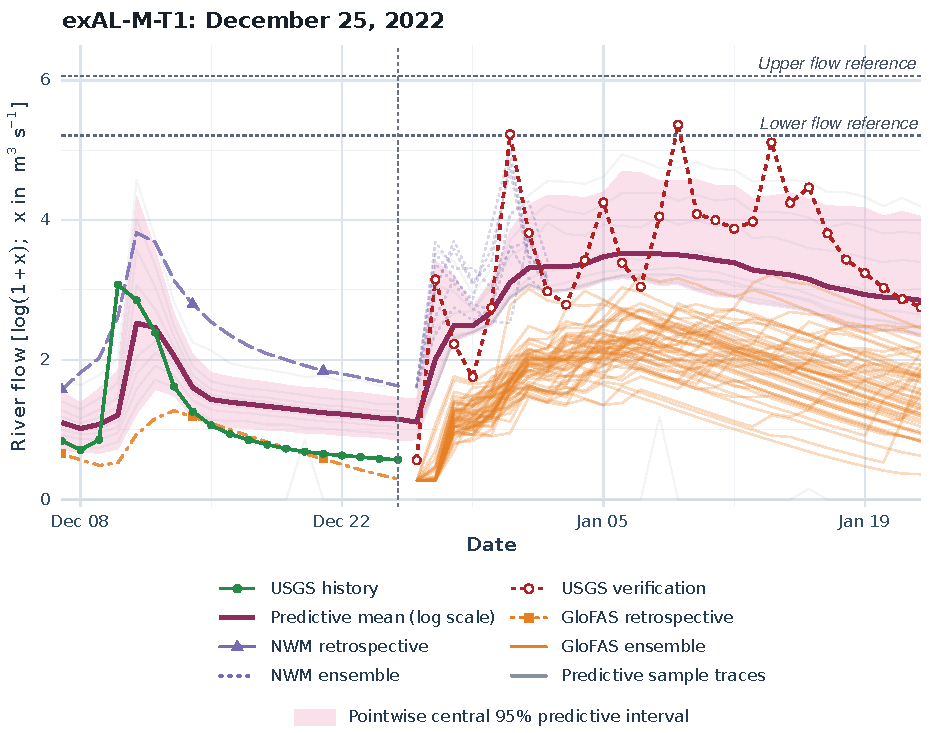
\includegraphics[width=0.95\textwidth]{figures/ch03-environ/predictive_synthesis_2022_12_25.pdf}
\caption[Predictive synthesis at the December 2022 origin]{Synthesized
exAL-M-T1 prediction at December 25, 2022, on the $\log(1+x)$ scale, with
$x$ in m$^3$/s. The 19 historical and 28 forecast dates show historical
observations and held-out verification values. The origin is $T$ and the first
lead is $T+1$. The maroon line is the predictive mean, the pink band is the
pointwise central 95\% predictive interval, and ten gray traces connect
predictive sample values within each period. GloFAS and NWS/NWM products give
source context. Horizontal guides mark approximately 182 and 429~m$^3$/s.}
\label{env:fig:synth1}
\end{figure}

\subsection{Distributional forecast performance}
\label{env:subsec:benchmarkresults}

Table~\ref{tab:external_benchmarks} compares the nine Bayesian configurations
and external references. The exAL-M-T1 mean-score reductions relative to
climatology are 68.6\% over 28 days and 59.0\% over eight days. EMOS-GLOFAS
also improves on climatology, with skill 0.288 and 0.391; persistence has
negative skill at both horizons. Raw NWS is scored only over its eight valid
daily leads.

% Generated by scripts/compact_publication.py; edit the generator.
\begin{table}[!htbp]
\centering
\begin{threeparttable}
\caption{Mean forecast CRPS and skill relative to seasonal climatology across five origins.}
\label{tab:external_benchmarks}
\setlength{\tabcolsep}{4pt}
\begin{tabular}{lrrrr}
\hline
Method & 28-day CRPS & 28-day CRPSS & 8-day CRPS & 8-day CRPSS \\
\hline
N-U-T1 & 0.87008 & -0.35489 & 0.99005 & -0.35752 \\
N-M-T0 & 0.83948 & -0.30723 & 0.72381 & 0.00755 \\
N-M-T1 & 2.38126 & -2.70811 & 3.18134 & -3.36211 \\
AL-U-T1 & 0.60367 & 0.05997 & 0.34086 & 0.53263 \\
AL-M-T0 & 0.53820 & 0.16192 & 0.61368 & 0.15855 \\
AL-M-T1 & 0.23230 & 0.63826 & 0.30944 & 0.57570 \\
exAL-U-T1 & 0.59631 & 0.07143 & 0.35144 & 0.51812 \\
exAL-M-T0 & 1.13760 & -0.77147 & 1.13421 & -0.55518 \\
exAL-M-T1 & \textbf{0.20164} & \textbf{0.68601} & \textbf{0.29926} & \textbf{0.58967} \\
GloFAS & 0.61761 & 0.03826 & 0.77502 & -0.06267 \\
NWS & --- & --- & 0.66478 & 0.08848 \\
Seasonal climatology & 0.64218 & 0.00000 & 0.72931 & 0.00000 \\
Persistence & 0.91061 & -0.41801 & 0.99854 & -0.36915 \\
GloFAS EMOS & 0.45734 & 0.28782 & 0.44450 & 0.39052 \\
\hline
\end{tabular}
\begin{tablenotes}\footnotesize
\item \textit{Note:} Scores use $\log(1+x)$ discharge, with $x$ in m$^3$/s. CRPS denotes the continuous ranked probability score; lower values are better. CRPSS is one minus the ratio of pooled mean CRPS to the matching climatology mean; higher values are better. Bold indicates the lowest CRPS or highest CRPSS in each column. Means use 140 daily cases at leads 1--28 and 40 at leads 1--8. NWS has eight daily leads. Scores use quantile-grid integration. N, AL and exAL denote normal, asymmetric Laplace and extended asymmetric Laplace likelihoods; U and M denote one and multiple observation sources. T1 retains the transfer contribution at forecast leads and T0 omits it.
\end{tablenotes}
\end{threeparttable}
\end{table}


Within AL and exAL models, source inclusion and retention of forecast transfer
improve 28-day CRPS at every origin. The exAL-M-T1 model has the lowest score
among the nine Bayesian variants and raw products at all five 28-day origins.
That comparison does not extend uniformly to every likelihood and horizon:
N-M-T1 is worse than N-M-T0 at every origin, and the best eight-day method
varies by origin. Raw NWS has the lowest score in December 2021 and December
2022, AL-U-T1 in January 2021, and exAL-M-T1 in November 2021 and May 2022.

EMOS-GLOFAS has smaller CRPS than exAL-M-T1 in May 2022: 28-day CRPS is
0.01763 versus 0.02273, and eight-day CRPS is 0.02381 versus 0.02567. ExAL-M-T1 improves on
all three benchmarks at the other four origins. On the discharge scale,
exAL-M-T1 has the smallest aggregate 28-day CRPS, whereas raw NWS has the
smallest aggregate eight-day CRPS. Appendix~\ref{env:app:additional-results}
reports the origin-specific and discharge-scale values. These results support
a 28-day distributional improvement, not uniform dominance across origins,
horizons, scores, or scales.

\subsection{Quantile performance and calibration}

Table~\ref{tab:quantile_check_loss_pooled} reports pooled 28-day check losses
for four quantile-synthesis competitors. ExAL-M-T1 has the smallest losses at
probabilities 0.05--0.50, whereas AL-M-T1 is best at 0.65--0.95. The targeted
losses therefore qualify the distribution-wide CRPS comparison.

% Generated by scripts/compact_publication.py; edit the generator.
\begin{table}[!htbp]
\centering
\begin{threeparttable}
\caption{Mean daily quantile check loss pooled over five 28-day forecast windows.}
\label{tab:quantile_check_loss_pooled}
\setlength{\tabcolsep}{4pt}
\begin{tabular}{lrrrrrrr}
\hline
Method & $0.05$ & $0.20$ & $0.35$ & $0.50$ & $0.65$ & $0.80$ & $0.95$ \\
\hline
AL-M-T1 & 0.04276 & 0.11409 & 0.15984 & 0.18053 & \textbf{0.13195} & \textbf{0.10446} & \textbf{0.05429} \\
AL-U-T1 & 0.05315 & 0.16341 & 0.25617 & 0.32472 & 0.39242 & 0.44899 & 0.46090 \\
exAL-M-T1 & \textbf{0.03057} & \textbf{0.07927} & \textbf{0.11265} & \textbf{0.14553} & 0.15261 & 0.10976 & 0.05582 \\
exAL-U-T1 & 0.04985 & 0.15945 & 0.25790 & 0.32564 & 0.38671 & 0.43920 & 0.45631 \\
\hline
\end{tabular}
\begin{tablenotes}\footnotesize
\item \textit{Note:} Columns are target probabilities; each entry averages 140 archived daily losses. Lower values are better; bold marks the minimum in each column. Scores use $\log(1+x)$ discharge, with $x$ in m$^3$/s. N, AL and exAL denote normal, asymmetric Laplace and extended asymmetric Laplace likelihoods; U and M denote one and multiple observation sources. T1 retains the transfer contribution at forecast leads and T0 omits it.
\end{tablenotes}
\end{threeparttable}
\end{table}


Individual exAL-M-T1 predictive quantiles cross on 61 of 140 forecast dates;
neither their isotonic projection nor the final synthesis crosses. Its mean
check loss across seven probabilities decreases from 0.10058 to 0.09803 after
synthesis over 28 days and from 0.15069 to 0.14622 over eight days. This
improvement is not universal across competitors, so isotonic projection is
the ordering correction while synthesis is a separate predictive choice.

The exAL-M-T1 central 95\% interval covers 123/140 cases (87.9\%) over 28
days and 29/40 (72.5\%) over eight days (Table~\ref{tab:no_refit_calibration}).
AL-M-T1 intervals are wider, cover 132/140 and 35/40 cases, and have smaller
mean interval scores. Favorable mean CRPS for exAL-M-T1 therefore coexists
with undercoverage, especially at the two December eight-day origins.

% Generated by scripts/compact_publication.py; edit the generator.
\begin{table}[!htbp]
\centering
\begin{threeparttable}
\caption{Coverage, mean width and mean interval score of central 95\% observation predictive intervals.}
\label{tab:no_refit_calibration}
\setlength{\tabcolsep}{4pt}
\resizebox{\textwidth}{!}{%
\begin{tabular}{lrrrrrr}
\hline
Method & \multicolumn{3}{c}{28 days} & \multicolumn{3}{c}{8 days} \\
 & Covered & Width & Interval score & Covered & Width & Interval score \\
\hline
exAL-M-T1 & 123/140 & 0.88870 & 2.50218 & 29/40 & 0.88509 & 4.46293 \\
AL-M-T1 & 132/140 & 1.45845 & \textbf{2.44957} & 35/40 & 1.55141 & \textbf{2.81501} \\
exAL-U-T1 & 75/140 & 0.62726 & 18.92775 & 27/40 & 0.79108 & 7.71508 \\
AL-U-T1 & 67/140 & 0.54957 & 19.49073 & 24/40 & 0.89059 & 6.83147 \\
GloFAS & 48/140 & 1.09584 & 15.64795 & 1/40 & 0.64042 & 23.02593 \\
NWS & --- & --- & --- & 12/40 & 0.64615 & 19.54956 \\
Seasonal climatology & 132/140 & 2.91666 & 4.28318 & 39/40 & 2.74092 & 4.14775 \\
Persistence & 0/140 & 0.00000 & 36.42450 & 0/40 & 0.00000 & 39.94145 \\
GloFAS EMOS & 106/140 & 1.63599 & 10.26329 & 27/40 & 1.70634 & 8.68153 \\
\hline
\end{tabular}%
}
\begin{tablenotes}\footnotesize
\item \textit{Note:} Covered is the number of observations within the closed 2.5th--97.5th percentile interval divided by the case count. Width and interval score are averaged on the $\log(1+x)$ scale, with discharge $x$ in m$^3$/s. Bold marks the lowest interval score for each horizon. Persistence has zero width. Numerical quantile conventions are specified in Appendix~\ref{app:numericalprediction}. The monotone inverse transformation preserves coverage. N, AL and exAL denote normal, asymmetric Laplace and extended asymmetric Laplace likelihoods; U and M denote one and multiple observation sources. T1 retains the transfer contribution at forecast leads and T0 omits it.
\end{tablenotes}
\end{threeparttable}
\end{table}


Figure~\ref{env:fig:no-refit-reliability} gives pooled quantile reliability.
Over 28 days, exAL-M-T1 strict frequencies at probabilities 0.05, 0.50, and
0.95 are 6/140, 67/140, and 128/140. The upper frequency falls below nominal,
consistent with upper-tail misses.

\begin{figure}[!htbp]
\centering
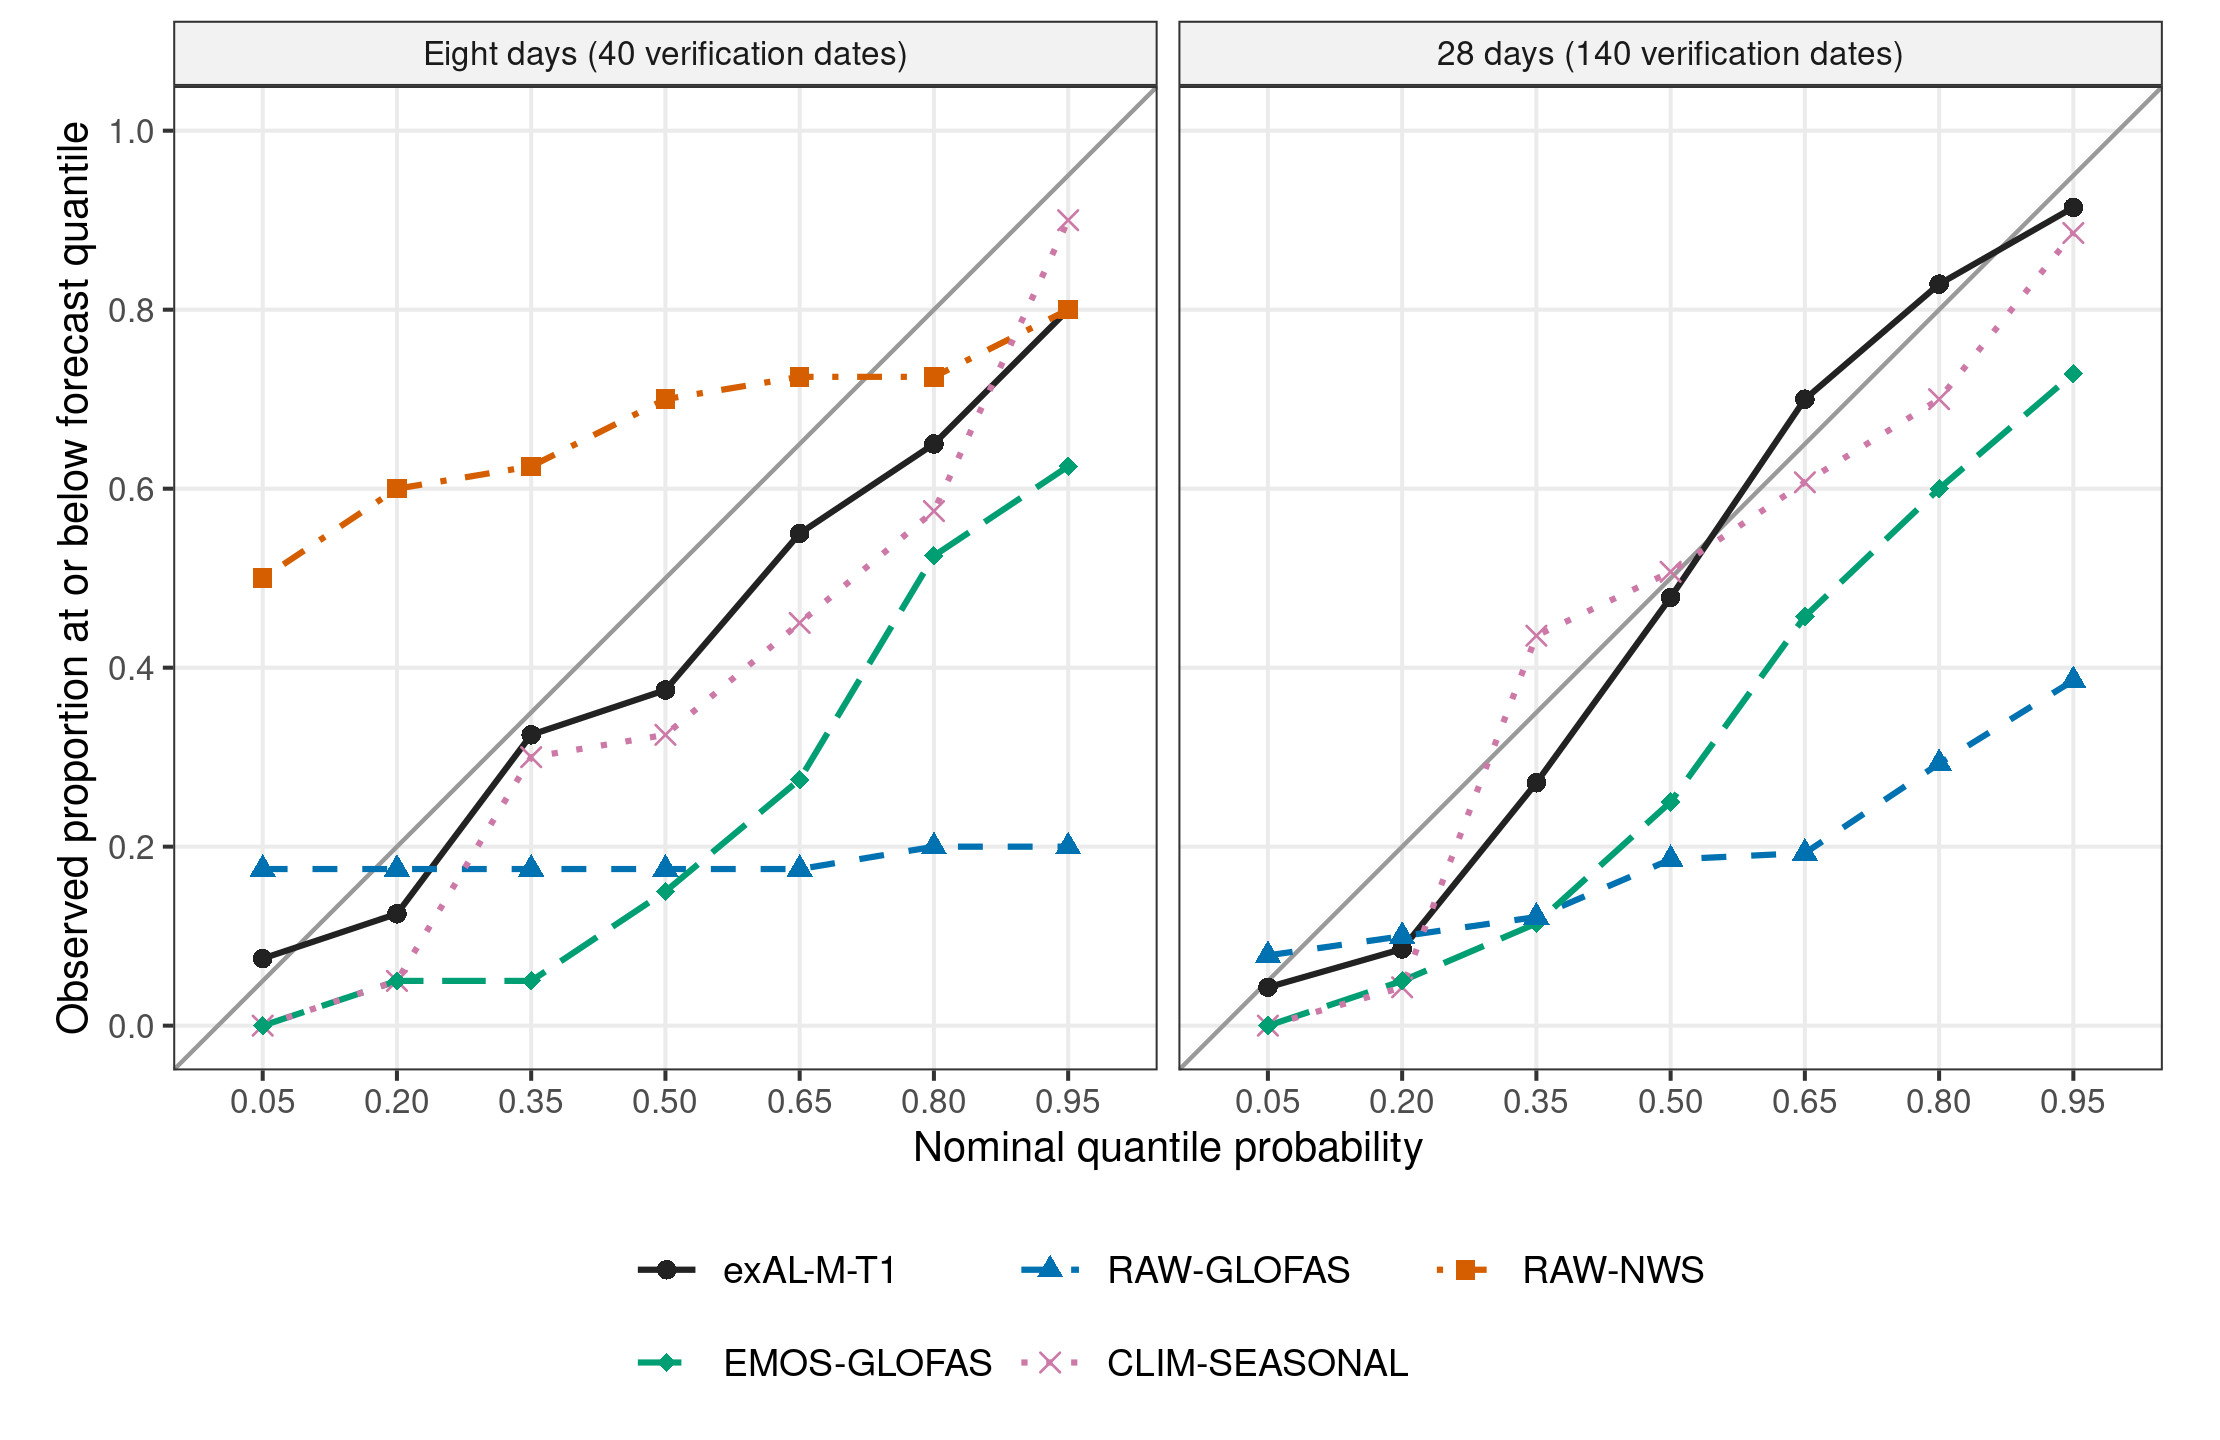
\includegraphics[width=0.92\textwidth]{figures/ch03-environ/no_refit_quantile_reliability.png}
\caption[Quantile reliability across forecast origins]{Quantile reliability
over eight and 28 days, pooling 40 and 140 cases across five origins. Curves
give frequencies at or below predictive quantiles for exAL-M-T1, raw
GloFAS/NWS, EMOS-GLOFAS, and seasonal climatology; the diagonal denotes
nominal probabilities. NWS is available over eight days.}
\label{env:fig:no-refit-reliability}
\end{figure}

\subsection{Component sensitivity and interpretation}
\label{env:sec:interpretation}

Each one-component reduction has higher CRPS than the full exAL-M-T1
specification and raw GloFAS at every origin over both horizons
(Table~\ref{tab:component_comparison}). These are sensitivity comparisons
under common fitting settings, not an exhaustive identification of the true
component structure. In May 2022, for example, the transfer-free fitted median
locations range from 10.53 to 10.81 against transformed verification values
of 0.42--0.57, illustrating the consequence of removing the transfer term in
that setting.

The transfer coefficients are conditional adjustments alongside source
products, discrepancies, seasonality, nonlinear terms, and lags; they have no
causal interpretation. Their variational credible intervals concern
parameters under an approximate posterior. The predictive intervals instead
concern future discharge observations and combine latent-state and parameter
uncertainty with observation variation and synthesis. Predictive agreement
does not establish accurate parameter credible intervals, and parameter
accuracy alone would not establish predictive calibration.

\section{Conclusions and limitations}
\label{env:sec5}

The shared dynamic quantile process corrects external products through
source-specific discrepancies while accommodating different forecast
horizons. Predictive synthesis uses the full distributions from separate
quantile fits, including their tails, to construct a nondecreasing marginal
quantile function. Joint scale--skewness updates through Laplace--Delta VB make
the extended-likelihood analysis feasible for the long daily record.

The clearest empirical gain is 28-day distributional prediction in the San
Lorenzo comparisons. ExAL-M-T1 reduces mean transformed-scale CRPS by 67.4\%
relative to raw GloFAS and 55.9\% relative to GloFAS EMOS. Its CRPS is smaller
than that of the other Bayesian variants at every 28-day origin and smaller
than that of EMOS at four of five origins; its aggregate 28-day advantage
persists on the discharge scale.
However, EMOS performs better in May 2022, raw NWS leads at two winter
eight-day origins, and AL-M-T1 has smaller pooled upper-quantile losses and
better interval calibration. The evidence therefore favors the fuller model
for the principal 28-day target while identifying material qualifications.

The analysis depends on aligned external products and supplied covariate
paths. The likelihood assumes conditionally independent member residuals and
shares source scales across leads. The five origins do not provide a dense
hindcast, and predictive performance does not validate the variational
posterior approximation. A controlled study comparing VB and MCMC under a
matched, computationally manageable model would separate parameter accuracy,
predictive agreement, and interval coverage. Further work could propagate
transfer-input uncertainty, model dependent quantiles jointly, enrich the
discrepancy structure, and extend the analysis to multiple gauges.
